\documentclass[12pt, a4paper]{report}
\usepackage[utf8]{inputenc}
\usepackage[english, russian]{babel}

\usepackage{graphicx}
\usepackage{listings}
\usepackage{color}

\usepackage{amsmath}
\usepackage{pgfplots}
\usepackage{url}
\usepackage{flowchart}
\usepackage{tikz}
\DeclareGraphicsExtensions{.pdf,.png,.jpg,.svg}
\usetikzlibrary{shapes, arrows}

\usepackage{pgfplotstable}

\renewcommand\contentsname{Содержание}

\usepackage{geometry}
\geometry{left=3cm}
\geometry{right=1cm}
\geometry{top=2cm}
\geometry{bottom=2cm}

\lstset{ %
language=C++,                 % выбор языка для подсветки (здесь это С)
basicstyle=\small\sffamily, % размер и начертание шрифта для подсветки кода
numbers=left,               % где поставить нумерацию строк (слева\справа)
numberstyle=\tiny,           % размер шрифта для номеров строк
stepnumber=1,                   % размер шага между двумя номерами строк
numbersep=-5pt,                % как далеко отстоят номера строк от         подсвечиваемого кода
backgroundcolor=\color{white}, % цвет фона подсветки - используем         \usepackage{color}
showspaces=false,            % показывать или нет пробелы специальными     отступами
showstringspaces=false,      % показывать или нет пробелы в строках
showtabs=false,             % показывать или нет табуляцию в строках
frame=single,              % рисовать рамку вокруг кода
tabsize=2,                 % размер табуляции по умолчанию равен 2 пробелам
captionpos=t,              % позиция заголовка вверху [t] или внизу [b] 
breaklines=true,           % автоматически переносить строки (да\нет)
breakatwhitespace=false, % переносить строки только если есть пробел
escapeinside={\%*}{*)},   % если нужно добавить комментарии в коде
keywordstyle=\color{blue}\ttfamily,
stringstyle=\color{red}\ttfamily,
commentstyle=\color{green}\ttfamily,
morecomment=[l][\color{magenta}]{\#},
columns=fullflexible }

\usepackage{titlesec}
\titleformat{\chapter}[hang]{\LARGE\bfseries}{\thechapter{.} }{0pt}{\LARGE\bfseries}
\titleformat*{\section}{\Large\bfseries}
\titleformat*{\subsection}{\large\bfseries}

\begin{document}

    \begin{titlepage}

        \begin{center}
            \Large
            {\sl Государственное образовательное учреждение высшего профессионального образования\\
            {\bf«Московский государственный технический университет имени Н.Э. Баумана»\\
				(МГТУ им. Н.Э. Баумана)}}
				\noindent\rule{\textwidth}{2pt}
            \vspace{3cm}

			{\scshape\LARGE Лабораторная работа №4 \par}
			\vspace{0.5cm}	
			{\scshape\LARGE по курсу «Анализ алгоритмов» \par}
			\vspace{1.5cm}
			{\huge\bfseries Распараллеливание алгоритма умножения матриц Винограда \par}
			\vspace{2cm}
			\Large Выполнил: Сорокин А.П., гр. ИУ7-52Б\\
			\vspace{0.5cm}
			{\Large Преподаватели: Волкова Л.Л., Строганов Ю.В.}
		
			\vfill
			\Large \textit {Москва, 2019 г.}
            
        \end{center}

    \end{titlepage}
	
	\tableofcontents

	\chapter*{Введение}
	\addcontentsline{toc}{chapter}{Введение}
	
	\hspace{1cm}В огромном количестве областей научной и технической сферы деятельности человека при различных математических расчетах используют такую операцию как умножение матриц. Это довольно трудоемкий процесс даже при небольших размерах матриц, так как требуется большое количество операций умножения и сложения различных чисел. По этой причине человек озадачен проблемой оптимизации умножения матриц и ускорения процесса вычисления.\\
	Таким образом, эффективное умножение матриц по времени и затратам ресурсов является актуальной проблемой для науки и техники.

    \chapter{Аналитическая часть}
	\section{Задачи}
	Цель лабораторной работы - изучение двух реализаций алгоритма умножения матриц Винограда: последовательной и параллельной.\\
	Для того чтобы добиться этой цели, были поставлены следующие задачи:
	\begin{itemize}
		\item изучить алгоритм Винограда;
		\item изучить методы параллельного программирования;
		\item применить знания программирования для реализации указанного алгоритма;
		\item выполнить сравнительный анализ последовательной реализации и параллельной реализации алгоритма Винограда при различном числе потоков;
		\item экспериментально подтвердить различия в эффективности по времени реализаций алгоритма Винограда.
	\end{itemize}

	\section{Описание алгоритмов}
	
	Матрицей называют математический объект, эквивалентный двумерному массиву. Матрица является таблицей, на пересечении строк и столбцов находятся элементы матрицы. Количество строк и столбцов является размерностью матрицы.\\
	Пусть даны две прямоугольные матрицы A и B размерности $m \times n$, $n \times q$
	соответственно:\\
	$$A =  \begin{bmatrix} 
	a_{11}& a_{12} &\ldots & a_{1n}\\ 
	a_{21}& a_{22} &\ldots & a_{2n}\\ 
	\vdots& \vdots &\ddots & \vdots\\ 
	a_{m1}& a_{m2} &\ldots & a_{mn} 
	\end{bmatrix} $$\\	
	
	$$B = \begin{bmatrix} 
	b_{11}& b_{12} &\ldots & b_{1q}\\ 
	b_{21}& b_{22} &\ldots & b_{2q}\\ 
	\vdots& \vdots &\ddots & \vdots\\ 
	b_{n1}& b_{n2} &\ldots & b_{nq} 
	\end{bmatrix} $$\\
	
	Тогда произведением матриц A и B называется матрица C размерностью  $m \times q$ \cite{Belousov}
	\begin{equation}
	\label{matrix-mult}
	C = \begin{bmatrix} 
	c_{11} & c_{12} & \cdots & c_{1q} \\
	c_{21} & c_{22} & \cdots & c_{2q} \\ 
	\vdots & \vdots & \ddots & \vdots \\ 
	c_{m1} & c_{m2} & \cdots & c_{mq}	
	\end{bmatrix}, ~\cite{CompAlg}
	\end{equation}
	в которой:
	$$c_{ij} = \sum_{k=1}^n a_{ik}b_{kj} \;\;\; \left(\overline{i = 1 \ldots m};\;\overline{j = 1 \ldots q} \right).$$

	\subsection{Алгоритм Винограда}
	Исходя из равенства \ref{matrix-mult}, видно, что каждый элемент в нем представляет собой скалярное произведение соответствующих строки и столбца исходных матриц. Такое умножение допускает предварительную обработку, позволяющую часть работы выполнить заранее. ~\cite{Winograd}\\
	Рассмотрим два вектора U и V:
	
	\begin{equation}
	\label{u-def}
	U = A_{i} = (u_{1}, u_{2}, \ldots, u_{n}),
	\end{equation}
	где $U = A_{i}$ -- i-ая строка матрицы A,\\
	$u_{k} = a_{ik}, \overline{k = 1 \ldots n}$ -- элемент i-ой строки k-ого столбца матрицы A.\\
	
	\begin{equation}
	\label{v-def}
	V = B_{j} = (v_{1}, v_{2}, \ldots, v_{n}),
	\end{equation}
	где $V = B_{j}$ -- j-ый столбец матрицы B,\\
	$v_{k} = b_{kj}, \overline{k = 1 \ldots n}$ -- элемент k-ой строки j-ого столбца матрицы B.\\
	
	По определению их скалярное произведение равно:\\
	\begin{equation}
	\label{uv-def}
	U \cdot V = u_{1}v_{1} + u_{2}v_{2} + u_{3}v_{3} + u_{4}v_{4}.
	\end{equation}
	Равенство \ref{uv-def} можно переписать в виде:\\
	\begin{equation}
	\label{uv}
	U \cdot V = (u_{1} + v_{2})(u_{2} + v_{1}) + (u_{3} + v_{4})(u_{4} + v_{3}) - u_{1}u_{2} - u_{3}u_{4} - v_{1}v_{2} - v_{3}v_{4}.
	\end{equation}
	В равенстве \ref{uv-def} насчитывается 4 операции умножения и 3 операции сложения, в равенстве \ref{uv} насчитывается 6 операций умножения и 9 операций сложения. Однако выражение $- u_{1}u_{2} - u_{3}u_{4}$ используются повторно при умножении i-ой строки матрицы A на каждый из столбцов матрицы B, а выражение $- v_{1}v_{2} - v_{3}v_{4}$ - при умножении j-ого столбца матрицы B на строки матрицы A. Таким образом, данные выражения можно вычислить предварительно для каждых строк и столбцов матриц для сокращения повторных вычислений. В результате повторно будут выполняться лишь 2 операции умножения и 7 операций сложения (2 операции нужны для добавления предварительно посчитанных произведений).
	
	\subsection{Параллельная реализация алгоритма Винограда}
	Трудоёмкость алгоритма Винограда для матриц размеров $M \times N$ и $N \times Q$ имеет сложность $O(MNQ)$. Для улучшения работы алгоритма необходимо выполнить распараллеливание той части алгоритма, которая задаёт данную сложность - часть, содержащая 3 вложенных цикла по размерам матриц.
	Вычисление результата для каждой строки результирующей матрицы не зависит от результата умножения других строк. Таким образом, можно выполнить распараллеливание той части кода, где выполняется вычисление строки. Вычисление отдельных групп строк результирующей матрицы будет отводиться под отдельный поток.
	
	\section{Параллельное программирование}
	При использовании многопроцессорных вычислительных систем с общей памятью обычно предполагается, что имеющиеся в составе системы процессоры обладают равной производительностью, являются равноправными при доступе к общей памяти, и время доступа к памяти является одинаковым (при одновременном доступе нескольких процессоров к одному и тому же элементу памяти очередность и синхронизация доступа обеспечивается на аппаратном уровне). Многопроцессорные системы подобного типа обычно именуются симметричными мультипроцессорами (symmetric multiprocessors, SMP).
	
	Перечисленному выше набору предположений удовлетворяют также активно развиваемые в последнее время многоядерные процессоры, в которых каждое ядро представляет практически независимо функциони рующее вычислительное устройство.
	
	Обычный подход при организации вычислений для многопроцессорных вычислительных систем с общей памятью – создание новых параллельных методов на основе обычных последовательных программ, в которых или автоматически компилятором, или непосредственно программистом выделяются участки независимых друг от друга вычислений. Возможности автоматического анализа программ для порождения параллельных вычислений достаточно ограничены, и второй подход является преобладающим. При этом для разработки параллельных программ могут применяться как новые алгоритмические языки, ориентированные на параллельное программирование, так и уже имеющиеся языки, расширенные некоторым набором операторов для параллельных вычислений.
	
	Широко используемый подход состоит и в применении тех или иных библиотек, обеспечивающих определенный программный интерфейс (application programming interface, API) для разработки параллельных программ. В рамках такого подхода наиболее известны Windows Thread API. Однако первый способ применим только для ОС семейства Microsoft Windows, а второй вариант API является достаточно трудоемким для использования и имеет низкоуровневый характер \cite{Barkalov}.
	
	\chapter{Конструкторская часть}
	
	\section{Схема алгоритма}
	На рисунке \ref{pic:vin} представлена схема оптимизированного алгоритма Винограда.
	\newpage
	\begin{figure}[ht!]
		\centering
		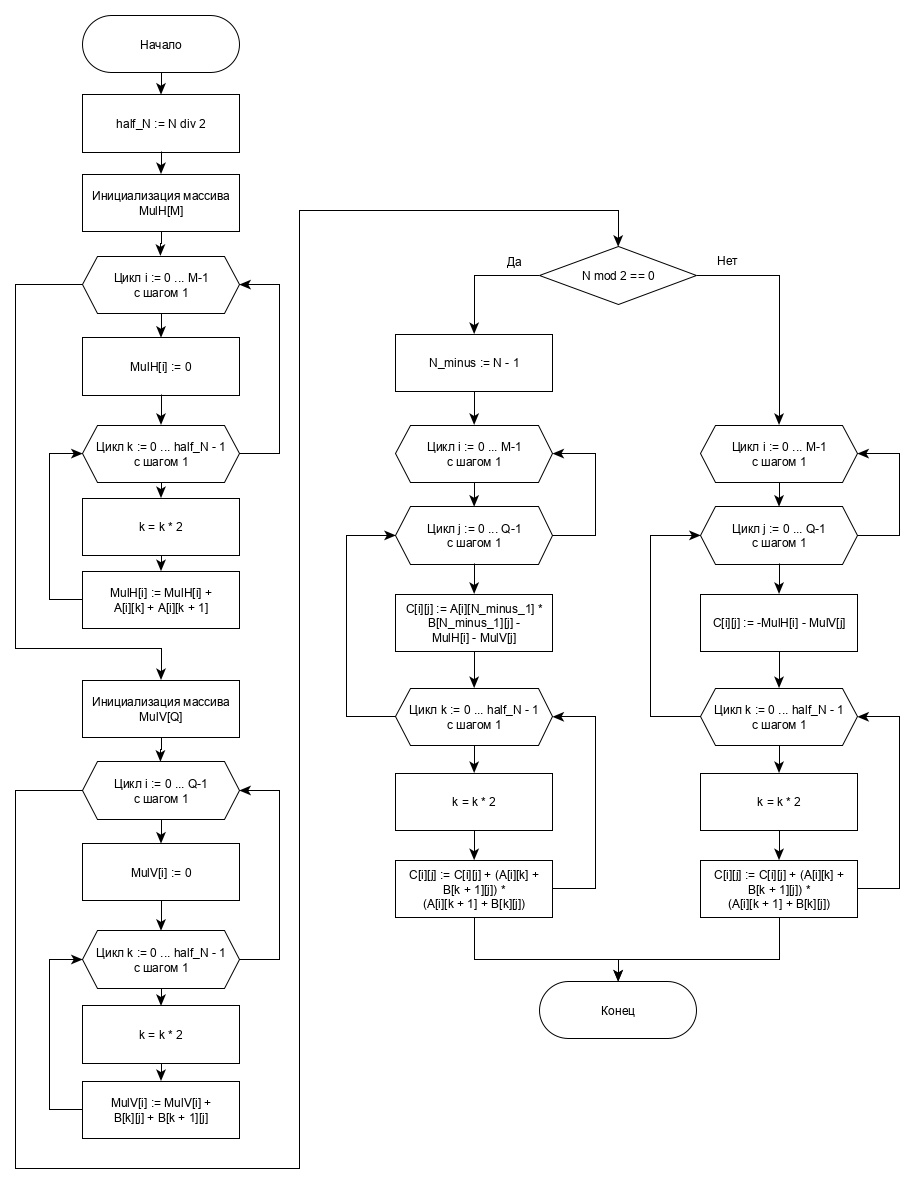
\includegraphics[scale=0.45]{vin.jpg}
		\caption{Алгоритм Винограда}
		\label{pic:vin}
	\end{figure}

	\newpage
	
	\section{Распараллеливание алгоритма}
	Распараллеливание алгоритма должно выполняться над теми данными, которые могут быть использованы только одним потоком. Это условие необходимо для обеспечения защиты данных от случайных изменений разными потоками одновременно. В данном алгоритме распараллеливание происходит в циклах, которые обозначены на схеме алгоритма участком A. В данных циклах каждая строка матрицы вычисляется независимо от других строк. Таким образом, многопоточность можно реализовать именно на данных циклах: каждый поток отвечает за определённые строки матрицы.
	
	Также можно выполнить параллельную инициализацию векторов MulV и MulH, так как инициализация их значений не зависят друг от друга.
	
	\chapter{Технологическая часть}
	\section{Требования к программному обеспечению}
	На вход подаются размеры двух матриц, затем число потоков для распараллеливания алгоритма. Матрицы генерируются случайным образом. На выход программа выдаёт сгенерированные исходные матрицы и результирующую матрицу.
	\section{Средства реализации}
	Для реализации программы был использован язык C++ ~\cite{CPP}. Для замера процессорного времени была использована функция rdtsc() из библиотеки stdrin.h. Потоки реализовывались с использованием библиотеки pthreads.h.
	\section{Реализации алгоритмов}
	В листинге \ref{code-seq} представлен код последовательной реализации алгоритма Винограда.
	\begin{lstlisting}[label=code-seq,caption=Последовательная реализация алгоритма Винограда]
	void multiply_vinograd_nothread(Matrix &A, Matrix &B)
	{
		const unsigned M = A.get_rows();
		const unsigned N = A.get_cols();
		const unsigned Q = B.get_cols();
		
		Matrix C(M, Q);
		
		unsigned half_N = N >> 1;
		
		int *MulH = new int[M];
		for (unsigned i = 0; i < M; i++)
		{
			MulH[i] = 0;
			for (unsigned k = 0; k < half_N; k++)
			{
				k <<= 1;
				MulH[i] += A[i][k] * A[i][k + 1];
			}
		}
		
		int *MulV = new int[Q];
		for (unsigned i = 0; i < Q; i++)
		{
			MulV[i] = 0;
			for (unsigned k = 0; k < half_N; k++)
			{
				k <<= 1;
				MulV[i] += B[k][i] * B[k + 1][i];
			}
		}
		
		if (N % 2)
		{
			unsigned N_minus_1 = N - 1;
			for (unsigned i = 0; i < M; i++)
				for (unsigned j = 0; j < Q; j++)
				{
					C[i][j] = A[i][N_minus_1] * B[N_minus_1][j] - MulH[i] - MulV[j];
					for (unsigned k = 0; k < half_N; k++)
					{
						k <<= 1;
						C[i][j] += (A[i][k] + B[k + 1][j]) * (A[i][k + 1] + B[k][j]);
					}
				}
		}
		else
		{
			for (unsigned i = 0; i < M; i++)
				for (unsigned j = 0; j < Q; j++)
				{
					C[i][j] = -MulH[i] - MulV[j];
					for (unsigned k = 0; k < half_N; k++)
					{
						k <<= 1;
						C[i][j] += (A[i][k] + B[k + 1][j]) * (A[i][k + 1] + B[k][j]);
					}
				}
		}
		
		delete [] MulH;
		delete [] MulV;
	}
	\end{lstlisting}
	
	\vspace{0.5cm}
	В листинге \ref{code-par} представлена параллельная реализация алгоритма Винограда.
	Функции потоков вычисления строк при чётных и нечётных размерах матриц представлены в листингах \ref{code-par-even} и \ref{code-par-odd} соответственно.
	Функции потоков инициализации рабочих векторов описаны в листинге \ref{code-par-vector}.
	Структура аргументов для функции потока описана в листинге \ref{code-par-args}.
	Структура класса "Матрица" описана в листинге \ref{code-matrix}.
	
	\begin{lstlisting}[label=code-matrix,caption=Класс Матрица]
	class Matrix;
	
	class Array
	{
	public:
		Array();
		explicit Array(unsigned size);
		Array(const Array& other);
	
		~Array();
	
		void alloc(unsigned size);
	
		void read(std::istream& stream);
		void write(std::ostream& stream);
	
		int& operator[](unsigned i);
	
		friend Matrix;
	
	private:
		int *ptr;
		unsigned _size;
	};
	
	class Matrix
	{
	public:
		Matrix(unsigned rows, unsigned cols);
		explicit Matrix(std::istream& stream);
		Matrix(const Matrix &other);
		~Matrix();
	
		void read(std::istream& stream);
		void write(std::ostream& stream);
	
		void randomize(int min, int max);
	
		Matrix& operator=(Matrix &other);
	
		bool operator==(const Matrix &other);
		bool operator!=(const Matrix &other);
	
		unsigned get_rows();
		unsigned get_cols();
		Array& operator[] (unsigned i);
	
	private:
		Array *ptr;
		unsigned _rows;
		unsigned _cols;
	};
	\end{lstlisting}
	
	\begin{lstlisting}[label=code-par-args,caption=Структура аргументов]
	typedef struct MultArgs_t
	{
		Matrix &A;
		Matrix &B;
		Matrix &C;
		int *MulH;
		int *MulV;
		unsigned half_N;
		unsigned N_minus_1;
		
		unsigned start_i;
		unsigned end_i;
	} MultArgs;
	
	typedef struct
	{
		int **MVector;
		Matrix &A;
		unsigned half_N;
	} InitVectorArgs;
	\end{lstlisting}
	
	\begin{lstlisting}[label=code-par,caption=Параллельная реализация алгоритма Винограда]
	Matrix multiply_vinograd_thread(Matrix &A, Matrix &B, unsigned thread_amount)
	{
		int status, status_addr;
		pthread_t thr_MulH, thr_MulV;
		pthread_t *threads = new pthread_t[thread_amount];
		
		const unsigned M = A.get_rows();
		const unsigned N = A.get_cols();
		const unsigned Q = B.get_cols();
		
		Matrix C(M, Q);
		
		unsigned half_N = N >> 1;
		
		int *MulH = nullptr, *MulV = nullptr;
		InitVectorArgs argsH = { &MulH, A, half_N };
		InitVectorArgs argsV = { &MulV, B, half_N };
		
		status = pthread_create(&thr_MulH, NULL, init_MultH, (void*) &argsH);
		if (status)
		{
			printf("Can't create thread for MulH, status = %d\n", status);
			exit(ERROR_CREATE_THREAD);
		}
		status = pthread_create(&thr_MulV, NULL, init_MultV, (void*) &argsV);
		if (status)
		{
			printf("Can't create thread for MulV, status = %d\n", status);
			exit(ERROR_CREATE_THREAD);
		}
		
		status = pthread_join(thr_MulH, (void**)&status_addr);
		if (status)
		{
			printf("Can't join thread thr_MulH, status = %d\n", status);
			exit(ERROR_JOIN_THREAD);
		}
		status = pthread_join(thr_MulV, (void**)&status_addr);
		if (status)
		{
			printf("Can't join thread thr_MulV, status = %d\n", status);
			exit(ERROR_JOIN_THREAD);
		}
		
		float step_i = M / float(thread_amount), value_i = step_i;
		unsigned start_i = 0, end_i = unsigned(value_i);
		
		std::vector<MultArgs> args;
		for (unsigned i = 0; i < thread_amount; i++)
		{
			args.push_back({A, B, C, MulH, MulV, half_N, N - 1, start_i, end_i});
			start_i = end_i;
			value_i += step_i;
			end_i = unsigned(value_i);
		}
		
		void* (*thread_func)(void*) = multiply_even;
		if (N % 2)
			thread_func = multiply_odd;
		
		for (unsigned i = 0; i < thread_amount; i++)
		{
			status = pthread_create(&(threads[i]), NULL, thread_func,
									(void*) &args[i]);
			if (status)
			{
				printf("Can't create thread %u, status = %d\n", i, status);
				exit(ERROR_CREATE_THREAD);
			}
		}
		
		for (unsigned i = 0; i < thread_amount; i++)
		{
			status = pthread_join(threads[i], (void**)&status_addr);
			if (status)
			{
				printf("Can't join thread %u, status = %d\n", i, status);
				exit(ERROR_JOIN_THREAD);
			}
		}
		
		delete [] MulH;
		delete [] MulV;
		delete [] threads;
		
		return C;
	}
	\end{lstlisting}
	
	\begin{lstlisting}[label=code-par-vector,caption=Функции потоков инициализации векторов]
	void *init_MultH(void *_args)
	{
		InitVectorArgs *args = (InitVectorArgs*) _args;
		
		const unsigned M = args->A.get_rows();
		*(args->MVector) = new int[M];
		for (unsigned i = 0; i < M; i++)
		{
			(*(args->MVector))[i] = 0;
			for (unsigned k = 0; k < args->half_N; k++)
			{
				k <<= 1;
				(*(args->MVector))[i] += args->A[i][k] * args->A[i][k + 1];
			}
		}
		return NULL;
	}
	
	void *init_MultV(void *_args)
	{
		InitVectorArgs *args = (InitVectorArgs*) _args;
		
		const unsigned Q = args->A.get_cols();
		*(args->MVector) = new int[Q];
		for (unsigned j = 0; j < Q; j++)
		{
			(*(args->MVector))[j] = 0;
			for (unsigned k = 0; k < args->half_N; k++)
			{
				k <<= 1;
				(*(args->MVector))[j] += args->A[k][j] * args->A[k + 1][j];
			}
		}
		return NULL;
	}
	\end{lstlisting}
	
	\begin{lstlisting}[label=code-par-even,caption=Функция потока вычисления строки при нечётных размерах матрицы]
	void *multiply_odd(void *_args)
	{
		MultArgs *args = (MultArgs*) _args;
		
		const unsigned Q = args->B.get_cols();
		
		for (unsigned i = args->start_i; i < args->end_i; i++)
			for (unsigned j = 0; j < Q; j++)
			{
				args->C[i][j] = args->A[i][args->N_minus_1] *
				args->B[args->N_minus_1][j]
				- args->MulH[i] - args->MulV[j];
				for (unsigned k = 0; k < args->half_N; k++)
				{
					k <<= 1;
					args->C[i][j] += (args->A[i][k] + args->B[k + 1][j]) *
									(args->A[i][k + 1] + args->B[k][j]);
				}
			}
		
		return NULL;
	}
	\end{lstlisting}
	
	\begin{lstlisting}[label=code-par-odd,caption=Функция потока вычисления строки при чётных размерах матрицы]
	void *multiply_even(void *_args)
	{
		MultArgs *args = (MultArgs*) _args;
		
		const unsigned Q = args->B.get_cols();
		
		for (unsigned i = args->start_i; i < args->end_i; i++)
			for (unsigned j = 0; j < Q; j++)
			{
				args->C[i][j] = -args->MulH[i] - args->MulV[j];
				for (unsigned k = 0; k < args->half_N; k++)
				{
					k <<= 1;
					args->C[i][j] += (args->A[i][k] + args->B[k + 1][j]) *
									(args->A[i][k + 1] + args->B[k][j]);
				}
			}
		
		return NULL;
	}
	\end{lstlisting}

	\newpage

	\section{Тесты}
	Для проверки корректности работы были подготовлены функциональные тесты, представленные в таблице \ref{unit-tests}. Входные данные удовлетворяют условиям, необходимым для умножения матриц, так как проверка на соответствие их размеров возложена на другую функцию.

	\begin{table}[ht!]
		\caption{Функциональные тесты}
		\label{unit-tests}
		\begin{center}
			\begin{tabular}{|c|c|c|}
			\hline
			\bf{Матрица 1} & \bf{Матрица 2} & \bf{Ожидание}\\\hline
			
			$\begin{bmatrix}5\end{bmatrix}$ &
			$\begin{bmatrix}-8\end{bmatrix}$ &
			$\begin{bmatrix}-40\end{bmatrix}$\\\hline
			
			$\begin{bmatrix}2 & 1 & 1\end{bmatrix}$ &
			$\begin{bmatrix}1\\-1\\5\end{bmatrix}$ &
			$\begin{bmatrix}6\end{bmatrix}$\\\hline
			
			$\begin{bmatrix}5 & 1\\0 & -1\end{bmatrix}$ &
			$\begin{bmatrix}3 & -5\\10 & 0\end{bmatrix}$ &
			$\begin{bmatrix}-10 & 25\\-10 & 0\end{bmatrix}$\\\hline
			
			$\begin{bmatrix}1 & 2 & 0\\3 & 0 & -1\end{bmatrix}$ &
			$\begin{bmatrix}1 & 2\\3 & 0\\0 & -2\end{bmatrix}$ &
			$\begin{bmatrix}7 & 2\\3 & 8\end{bmatrix}$\\\hline
			
			$\begin{bmatrix}1 & 1 & -1\\5 & -3 & -4\end{bmatrix}$ &
			$\begin{bmatrix}0 & 0\\0 & 0\\0 & 0\end{bmatrix}$ &
			$\begin{bmatrix}0 & 0\\0 & 0\end{bmatrix}$\\\hline
			
			$\begin{bmatrix}1 & 0\\0 & 1\end{bmatrix}$ &
			$\begin{bmatrix}1 & 3\\-2 & 1\end{bmatrix}$ &
			$\begin{bmatrix}1 & 3\\-2 & 1\end{bmatrix}$\\\hline

			\end{tabular}
		\end{center}
	\end{table}

	В результате проверки последовательная реализация алгоритма Винограда и его параллельная реализация при различном числе потоков прошли все поставленные функциональные тесты.

	\chapter{Экспериментальная часть}
	\section{Примеры работы}
	На рисунке \ref{pic:example} представлен пример работы программы, демонстрирующий корректную работу алгоритмов.
	\begin{figure}[ht!]
		\centering
		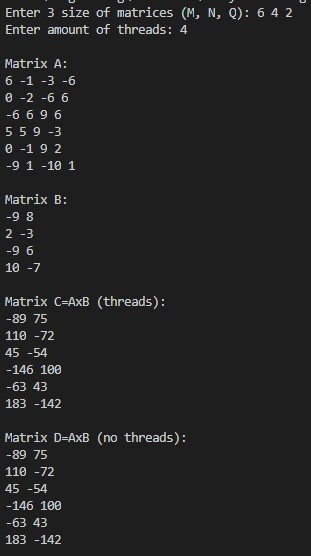
\includegraphics[scale=1]{example.jpg}
		\caption{Пример работы программы}
		\label{pic:example}
	\end{figure}
	
	\section{Сравнение работы алгоритмов при чётных размерах матрицы}
	Для сравнения времени работы алгоритмов умножения матриц были использованы квадратные матрицы размером от 100 до 1000 с шагом 100. Эксперимент для более точного результата повторялся 100 раз. Итоговый результат рассчитывался как средний из полученных результатов. Эксперимент проводился на компьютере с 4 логическими процессорами. Результаты измерений показаны в таблице \ref{table-even} и на рисунках \ref{graph-even} и \ref{graph-even-2}.\\
	\begin{table}[ht!]
		\caption{Время работы алгоритма при чётных размерах матриц}
		\label{table-even}
		\begin{center}
			\pgfplotstabletypeset[
			col sep=semicolon,
			string type,
			columns/Size/.style={column name=матриц, column type={|c}},
			columns/2/.style={column name=2 потоках, column type={|c}},
			columns/4/.style={column name=4 потоках, column type={|c}},
			columns/6/.style={column name=6 потоках, column type={|c}},
			columns/8/.style={column name=8 потоках, column type={|c}},
			columns/NonParallel/.style={column name=без потоков, column type={|c|}},
			every head row/.style={
				before row={
					\hline
					Размер &
					\multicolumn{4}{c|}{Время в тиках при} &
					\multicolumn{1}{c|}{Время в тиках}\\
				},
				after row=\hline
			},
			every last row/.style={after row=\hline},
			]{TEvenTime.csv}
		\end{center}
	\end{table}
	
	\begin{figure}[ht!]
		\begin{tikzpicture}
		\begin{axis}
			[%title = График времени работы алгоритмов при чётных размерах матриц,
			table/col sep = semicolon,
			xlabel={Размер матриц},
			ylabel={Время в тиках},
			ymin = 0,
			legend pos=outer north east,
			ymajorgrids=true,
			grid style=dashed]
			\addplot[color=red, mark=*] table[x={Size}, y={2}] {TEvenTime.csv};
			\addplot[color=blue, mark=*] table[x={Size}, y={4}] {TEvenTime.csv};
			\addplot[color=green, mark=*] table[x={Size}, y={6}] {TEvenTime.csv};
			\addplot[color=orange, mark=*] table[x={Size}, y={8}] {TEvenTime.csv};
			\legend{2 потока, 4 потока, 6 потоков, 8 потоков}
		\end{axis}
		\end{tikzpicture}
		\caption{График времени работы алгоритмов при чётных размерах матриц}
		\label{graph-even}
	\end{figure}
	
	Можно заметить, что с ростом числа используемых потоков, уменьшается и время работы алгоритма: время работы при 2 потоках в 2 раза больше времени работы при 4 потоках. Однако, время работы при 6 и 8 потоках приблизительно одинаково, при этом оно выше времени работы при 4 потоках: время работы при 6-8 потоках выше в среднем на 40\% по сравнению с временем при двух, причём время при восьми меньше, чем время при шести.
	Стоит заметить, что при размерах матриц, равным 1000, уже время при 6 потоках является самым минимальным: оно меньше времени при 4 потоках на 2,6\%. При этом время работы алгоритма при 8 потоках также меньше времени при двух (на 2,0\%).
	
	Наилучший результат показывает многопоточная реализация алгоритма, когда работает на 4 потоках. При этом стоит заметить, что число потоков 4 равно количеству логических процессоров используемого компьютера. Исходя из этого можно сделать вывод о том, что наилучшего времени работы многопоточной реализации алгоритма можно добиться при числе потоков, равному количеству логических процессоров.
	
	\begin{figure}[ht!]
		\begin{tikzpicture}
		\begin{axis}
		[%title = График времени работы алгоритмов при чётных размерах матриц,
		table/col sep = semicolon,
		xlabel={Размер матриц},
		ylabel={Время в тиках},
		ymin = 0,
		legend pos=outer north east,
		ymajorgrids=true,
		grid style=dashed]
		\addplot[color=red, mark=*] table[x={Size}, y={2}] {TEvenTime.csv};
		\addplot[color=blue, mark=*] table[x={Size}, y={4}] {TEvenTime.csv};
		\addplot[color=gray, mark=*] table[x={Size}, y={NonParallel}] {TOddTime.csv};
		\legend{2 потока, 4 потока, без потоков}
		\end{axis}
		\end{tikzpicture}
		\caption{График времени работы двух реализаций при чётных размерах матриц}
		\label{graph-even-2}
	\end{figure}
	
	Легко заметить, что многопоточная реализация даже в худшем случае (при 2 потоках) значительно выигрывает последовательную реализацию: последовательная реализация проигрывает в 1,6 раз многопоточной реализации при работе на 2 потоках, в 3 раза - при работе на 4 потоках.
	
	\section{Сравнение работы алгоритмов при нечётных размерах матрицы}
	Для сравнения времени работы алгоритмов умножения матриц были использованы квадратные матрицы размером от 101 до 1001 с шагом 100. Эксперимент для более точного результата повторялся 100 раз. Итоговый результат рассчитывался как средний из полученных результатов. Эксперимент проводился на компьютере с 4 логическими процессорами. Результаты измерений показаны в таблице \ref{table-odd} и на рисунках \ref{graph-odd} и \ref{graph-odd-2}.\\
	
	\begin{table}[ht!]
		\caption{Время работы алгоритма при нечётных размерах матриц}
		\label{table-odd}
		\begin{center}
			\pgfplotstabletypeset[
			col sep=semicolon,
			string type,
			columns/Size/.style={column name=матриц, column type={|c}},
			columns/2/.style={column name=2 потоках, column type={|c}},
			columns/4/.style={column name=4 потоках, column type={|c}},
			columns/6/.style={column name=6 потоках, column type={|c}},
			columns/8/.style={column name=8 потоках, column type={|c}},
			columns/NonParallel/.style={column name=без потоков, column type={|c|}},
			every head row/.style={
				before row={
					\hline
					Размер &
					\multicolumn{4}{c|}{Время в тиках при} &
					\multicolumn{1}{c|}{Время в тиках}\\
				},
				after row=\hline
			},
			every last row/.style={after row=\hline},
			]{TOddTime.csv}
		\end{center}
	\end{table}

	\begin{figure}[ht!]
		\begin{tikzpicture}
		\begin{axis}
		[%title = График времени работы алгоритмов при нечётных размерах матриц,
		table/col sep = semicolon,
		xlabel={Размер матриц},
		ylabel={Время в тиках},
		ymin = 0,
		legend pos=outer north east,
		ymajorgrids=true,
		grid style=dashed]
		\addplot[color=red, mark=*] table[x={Size}, y={2}] {TOddTime.csv};
		\addplot[color=blue, mark=*] table[x={Size}, y={4}] {TOddTime.csv};
		\addplot[color=green, mark=*] table[x={Size}, y={6}] {TOddTime.csv};
		\addplot[color=orange, mark=*] table[x={Size}, y={8}] {TOddTime.csv};
		\legend{2 потока, 4 потока, 6 потоков, 8 потоков}
		\end{axis}
		\end{tikzpicture}
		\caption{График времени работы многопоточной реализации при нечётных размерах матриц}
		\label{graph-odd}
	\end{figure}

	\begin{figure}[ht!]
		\begin{tikzpicture}
		\begin{axis}
		[%title = График времени работы алгоритмов при нечётных размерах матриц,
		table/col sep = semicolon,
		xlabel={Размер матриц},
		ylabel={Время в тиках},
		ymin = 0,
		legend pos=outer north east,
		ymajorgrids=true,
		grid style=dashed]
		\addplot[color=red, mark=*] table[x={Size}, y={2}] {TOddTime.csv};
		\addplot[color=blue, mark=*] table[x={Size}, y={4}] {TOddTime.csv};
		\addplot[color=gray, mark=*] table[x={Size}, y={NonParallel}] {TOddTime.csv};
		\legend{2 потока, 4 потока, без потоков}
		\end{axis}
		\end{tikzpicture}
		\caption{График времени работы двух реализаций при нечётных размерах матриц}
		\label{graph-odd-2}
	\end{figure}
	
 	При нечётных размерах матриц разница во времени при работе алгоритма при разном числе потоков и в сравнении с последовательной реализацией та же, что и при чётных размерах матриц.

	\chapter*{Заключение}
	\addcontentsline{toc}{chapter}{Заключение}
	В ходе лабораторной работы был рассмотрен алгоритм Винограда и возможность его оптимизации путём распараллеливания алгоритм с помощью потоков.\\
	
	Была рассмотрена технология параллельного программирования и организация взаимодействия параллельных потоков. Потоки исполняются в общем адресном пространстве параллельной программы. Как результат, взаимодействие параллельных потоков можно организовать через использование общих данных, являющихся доступными для всех потоков. Наиболее простая ситуация состоит в использовании общих данных только для чтения. В случае же, когда общие данные могут изменяться несколькими потоками, необходимы специальные усилия для организации правильного взаимодействия. В данной лабораторной работе в качестве данных для чтения использовались исходные матрицы, которые требуется перемножить, а в качестве данных для записи - результирующая матрица, причём потоки обрабатывал только свои диапазоны строк, которые не пересекались.\\
	
	В ходе работы экспериментально была подтверждена эффективность многопоточной реализацией над последовательной, а также был проведён сравнительный анализ времени работы при различном числе потоков. Был сделан вывод о том, что наиболее оптимальное количество потоков в программе должно соответствовать количеству логических процессоров используемого компьютера.
	
	\newpage
	
	\begin{thebibliography}{}
	\bibitem{Belousov}И. В. Белоусов(2006), Матрицы и определители, учебное пособие по линейной алгебре, с. 1 - 16
	\bibitem{Winograd} Jelfimova L. A new fast systolic array for modified Winograd algorithm // Proc. Sevens Int. Workshop on Parallel Processing by Cellular Automata and Array, PARCELLA-96 (Berlin, Germany, Sept. 1996). — Berlin: Akad. Verlag. — 1996.
	\bibitem{Barkalov} Константин Баркалов, Владимир Воеводин, Виктор Гергель. Intel Parallel Programming [Электронный ресурс], - режим доступа
	\bibitem{CPP} https://cppreference.com/ [Электронный ресурс]
	\end{thebibliography}
	\addcontentsline{toc}{chapter}{Литература}

\end{document}
